%%%%%%%%%%%%%%%%%%%%%%%%%%%%%%%%%%%%%
%%%%%%%%%%%%            PREAMBLE          %%%%%%%%%%%%
%%%%%%%%%%%%%%%%%%%%%%%%%%%%%%%%%%%%%

\documentclass[aspectratio=169, xcolor=dvipsnames]{beamer}
\usecolortheme[named=Red]{structure} 
\usepackage{graphicx}
\usepackage{subcaption}

%%%%%%%%%%%%%%%%%%%%%%%%%%%%%%%%%%%%
%%%%%%%%%%%%           TITLE PAGE         %%%%%%%%%%%
%%%%%%%%%%%%%%%%%%%%%%%%%%%%%%%%%%%%

\title[]{Poverty Mapping in Off-Census Years}

\date{\today}

\author[]{Paul Corral, Heath Henderson, and Sandra Segovia \newline
~ \newline
World Bank Summer University 2024}

\begin{document}

%%%%%%%%%%%%%%%%%%%%%%%%%%%%%%%%%%%%
%%%%%%%%%%%%%           CONTENT         %%%%%%%%%%%
%%%%%%%%%%%%%%%%%%%%%%%%%%%%%%%%%%%%

% Title slide
\begin{frame}
\titlepage
\end{frame}

% Introduction
\begin{frame}{Introduction}
\begin{itemize}
\item Recent developments in poverty mapping in off-census years have
departed from standard practice in important ways.
\item In brief, standard practice consists of two basic steps:
\begin{enumerate}
\item Fit a parametric statistical model by regressing a survey-based 
welfare measure on some area-level covariates, typically census aggregates.
\item Predict the welfare measure for all geographic entities using the census
aggregates.
\end{enumerate}
\item In contrast to this ``traditional'' approach, the ``modern'' approach:
\begin{enumerate}
\item Relies on non-parametric, machine-learning methods rather than 
parametric models
\item Tends to rely more on non-traditional, remotely-sensed covariates in the estimation and
prediction stage
\end{enumerate}
\item In what follows, we'll discuss this modern approach in more detail and 
work through a simple application.
\end{itemize}
\end{frame}

% An Example
% Note: Chi et al. produce wealth estimates for the populated surface of all 135 
% LMICs at 2.4 km resolution. They rely heavily on machine learning and remotely-sensed
% data to produce their estimates.
\begin{frame}{An Example}
\begin{figure}[h!]
  \centering
  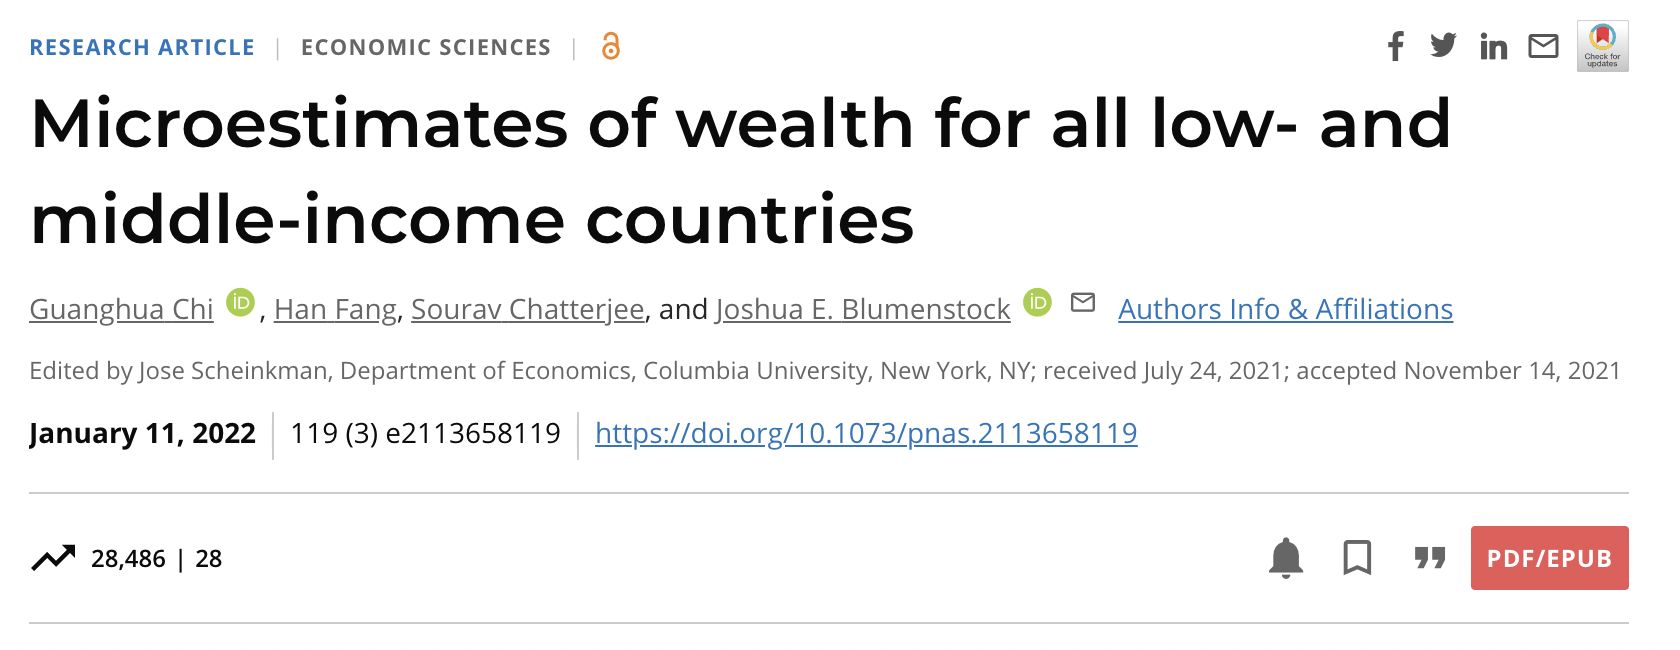
\includegraphics[width=0.8 \textwidth]{Chi_1}
\end{figure}
\end{frame}

% An Example
% Note: Panel A shows the 56 countries with available Demographic and Health
% Survey (DHS) data. Panel B shows an example of the survey coverage for
% one of the countries: Nigeria. Between 20 and 50 surveys were conducted in 
% each area ("village") and they used these surveys to calculate the average
% relative wealth for each. Panel C shows the remotely-sensed data that they
% matched to each village. After fitting a gradient boosting model to these data,
% they used to model to predict relative wealth for all 135 countries at 2.4 km
% resolution.
\begin{frame}{An Example}
\begin{figure}[h!]
  \centering
  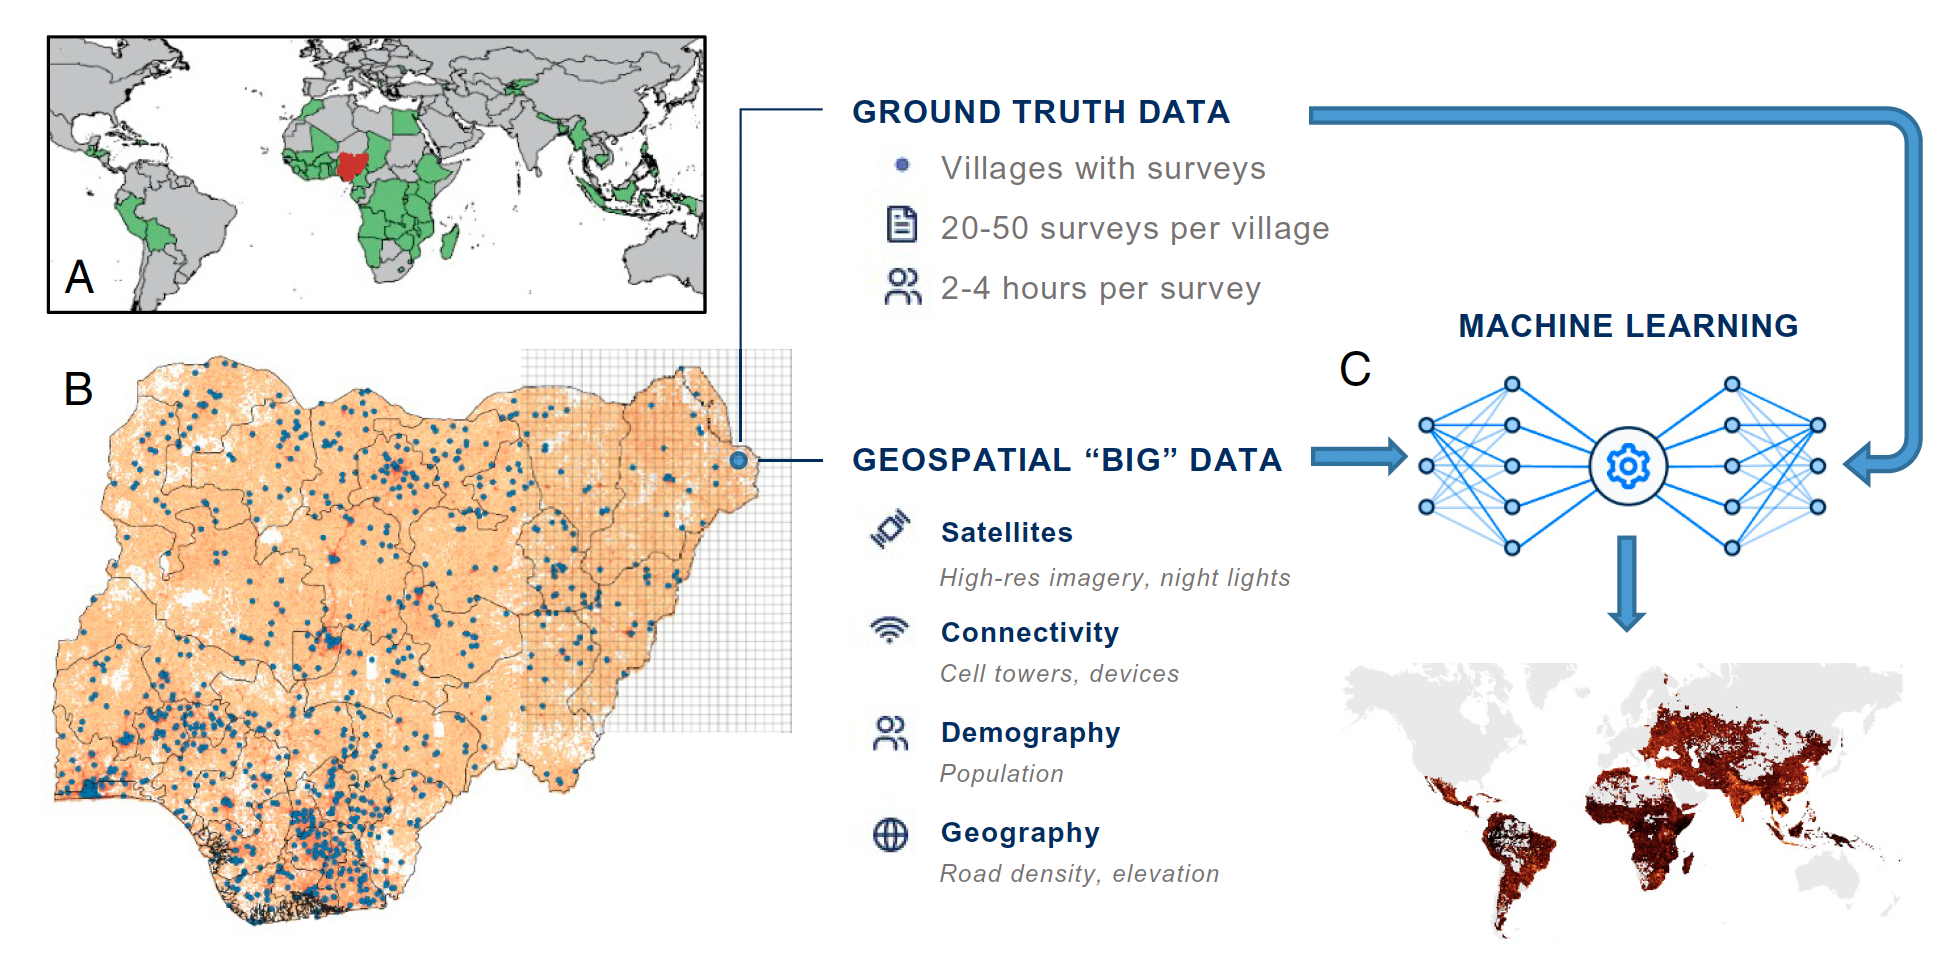
\includegraphics[width=0.8 \textwidth]{Chi_2}
\end{figure}
\end{frame}

% An Example
% Note: The inset shows South Africa and Lesoto.
\begin{frame}{An Example}
\begin{figure}[h!]
  \centering
  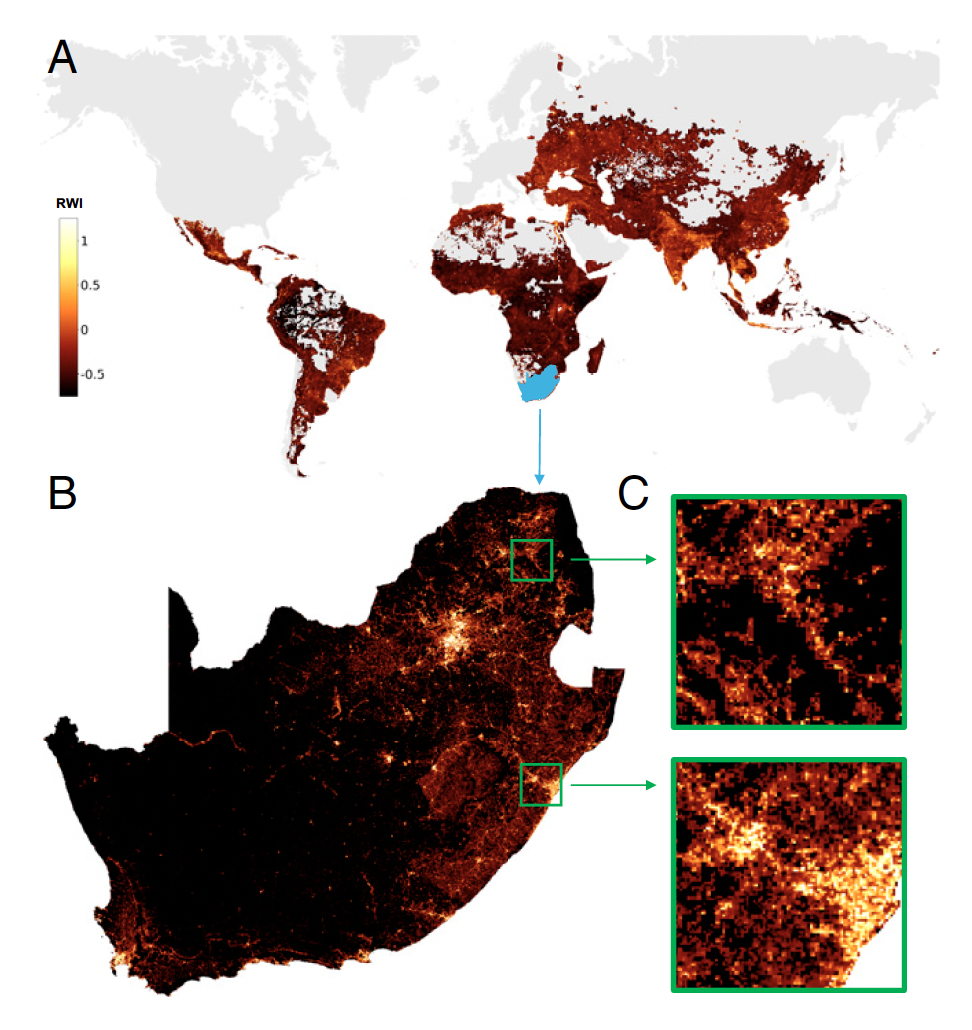
\includegraphics[width=0.45 \textwidth]{Chi_3}
\end{figure}
\end{frame}

% Machine Learning
\begin{frame}{Machine Learning}
\begin{itemize}
\item Machine learning plays a critical role in the modern approach to poverty 
mapping.
\item The goal of machine learning is to develop high-performance algorithms for 
prediction, classification, and clustering/grouping tasks.
\item Broadly speaking, machine-learning methods can be divided into two basic types:
\begin{enumerate}
\item Unsupervised learning: Seeks to identify clusters of observations that are
similar
\item Supervised learning: Uses a set of features to predict some outcome of
interest
\end{enumerate}
\item Supervised learning can be further divided into regression and classification tasks:
\begin{enumerate}
\item Regression: Concerned with predicting continuous outcomes
\item Classification: Focuses on predicting categorical outcomes
\end{enumerate}
\end{itemize}
\end{frame}

% Machine Learning
\begin{frame}{Machine Learning}
\begin{itemize}
\item There are many machine-learning methods for regression and classification 
(e.g., random forests, support vector machines, or Bayesian additive regression trees).
\item To fix ideas, we'll focus on one method that's been especially popular for poverty
mapping: gradient boosting.
\item Gradient boosting machines combine a large number of weak ``learners'' to form
a stronger ``ensemble'' prediction:
\begin{itemize}
\item Models are added to the ensemble sequentially by fitting new learners to the 
negative gradient of the loss function.
\item With a squared-error loss function, this amounts to sequentially fitting new models
to the current residuals of the ensemble.
\end{itemize}
\item Extreme gradient boosting (XGBoost) is a particularly popular implementation
that uses classification and regression trees as the base models.
\end{itemize}
\end{frame}

% Machine Learning
\begin{frame}{Machine Learning}
\begin{figure}
\begin{subfigure}[h]{0.4\linewidth}
\includegraphics[width=\linewidth]{tree}
\caption{Regression tree}
\end{subfigure}
\hspace{10pt}
\begin{subfigure}[h]{0.4\linewidth}
\includegraphics[width=\linewidth]{partition}
\caption{Covariate space}
\end{subfigure}
\end{figure}
\end{frame}

% Machine Learning
\begin{frame}{Machine Learning}
\begin{itemize}
\item For any given observation, the ensemble prediction used by XGBoost is the
sum of that observation's predictions across all trees in the ensemble:
\begin{equation*}
y_i^p = \sum_t f_t(x_i)
\end{equation*}
\item To build the trees in the ensemble, XGBoost minimizes the following objective function:
\begin{equation*}
\sum_i l(y_i^d, y_i^p) + \sum_t r(f_t)
\end{equation*}
\item XGBoost uses the following specification for the regularization term:
\begin{equation*}
r(f_t) = \gamma M_t + \frac{1}{2}\lambda \sum_j m_{tj}^2
\end{equation*}
\end{itemize}
\end{frame}

% Machine Learning
\begin{frame}{Machine Learning}
\begin{itemize}
\item To minimize the objective function, the model is trained in a sequential 
manner, building one tree at a time.
\item Ideally, one would select trees by enumerating all possible structures and then
using the one that minimizes the objective function, but this is often intractable.
\item XGBoost instead seeks to minimize the objective function by greedily optimizing
one level of the tree at a time:
\begin{enumerate}
\item For a given node, calculate the reduction in the objective function for every possible 
split rule for every available covariate.
\item Split the node using the covariate and split rule that maximally reduces the 
objective function.
\end{enumerate}
\item XGBoost continues splitting nodes until some user-specified stopping rule is
met.
\end{itemize}
\end{frame}

% Machine Learning
\begin{frame}{Machine Learning}
\begin{itemize}
\item Like many machine-learning models, XGBoost relies on various 
hyperparameters that must be selected by the user:
\begin{itemize}
\item The regularization term (i.e., $\gamma$ and $\lambda$)
\item Maximum tree depth and number of trees
\item Feature subsampling
\item The learning rate
\end{itemize}
\item There are several different ways one might approach hyperparameter selection:
\begin{itemize}
\item Use the default hyperparameters
\item Grid search
\item Bayesian hyperparameter optimization
\end{itemize}
\end{itemize}
\end{frame}

% An Application
\begin{frame}{An Application}
\begin{itemize}
\item Poverty maps in off-census years are generally produced with two types
of data:
\begin{itemize}
\item Direct poverty estimates for a subset of areas
\item A list of covariates or predictors for all areas
\end{itemize}
\item For a simple application, we'll use the 2015 Mexican Intercensal Survey (MIS)
for both data sources:
\begin{itemize}
\item The sample consists of 5.9 million households
\item Representative at the national, state, and municipality level
\item Gathered information on household income, location, demographics, etc.
\end{itemize}
\item We'll treat the MIS as if it were a real census and use it to simulate the
data used for poverty maps in off-census years:
\begin{itemize}
\item Sample households from the MIS to obtain direct poverty estimates for a 
subset of municipalities.
\item Collapse the micro-data to the municipality level to obtain area-level covariates.
\end{itemize}
\end{itemize}
\end{frame}

% An Application
\begin{frame}{An Application}
\begin{figure}[h!]
  \centering
  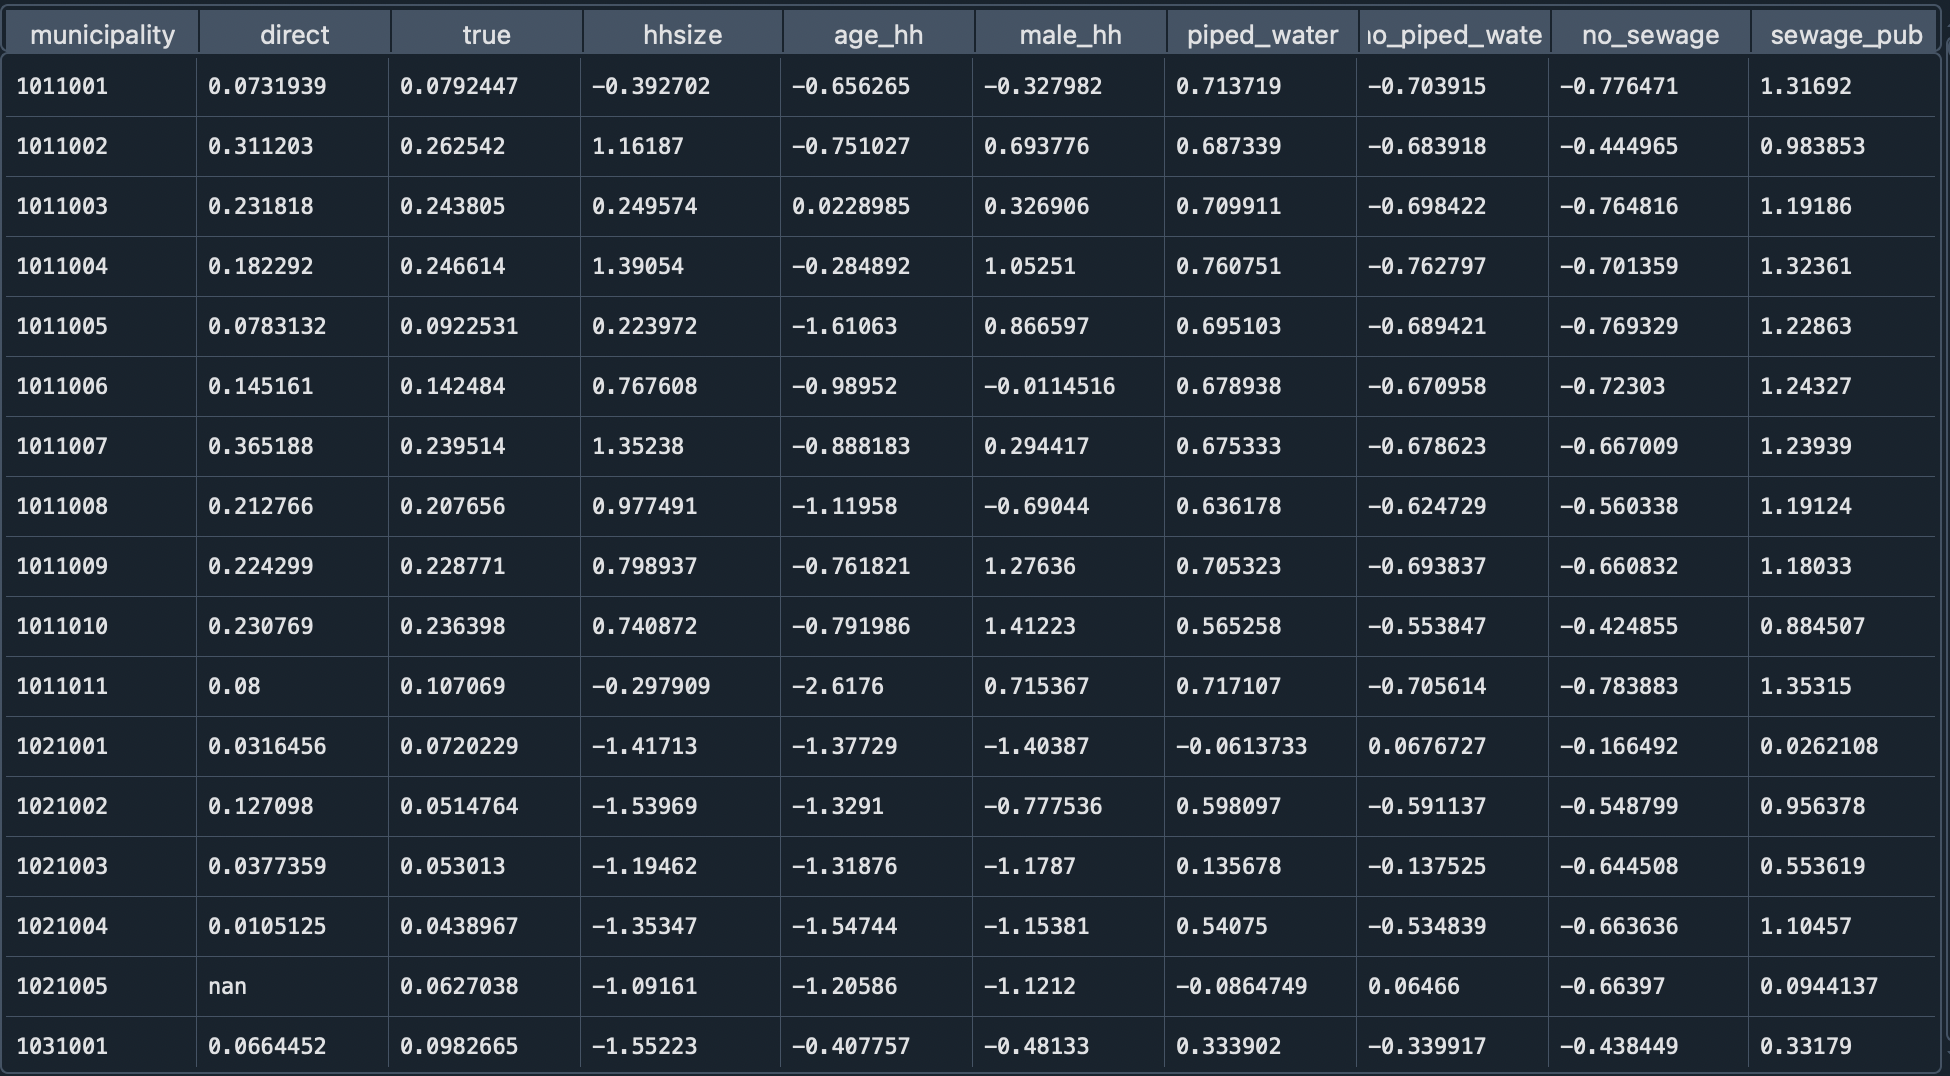
\includegraphics[width=0.7 \textwidth]{Data}
\end{figure}
\end{frame}

% An Application
\begin{frame}{An Application}
\begin{figure}[h!]
  \centering
  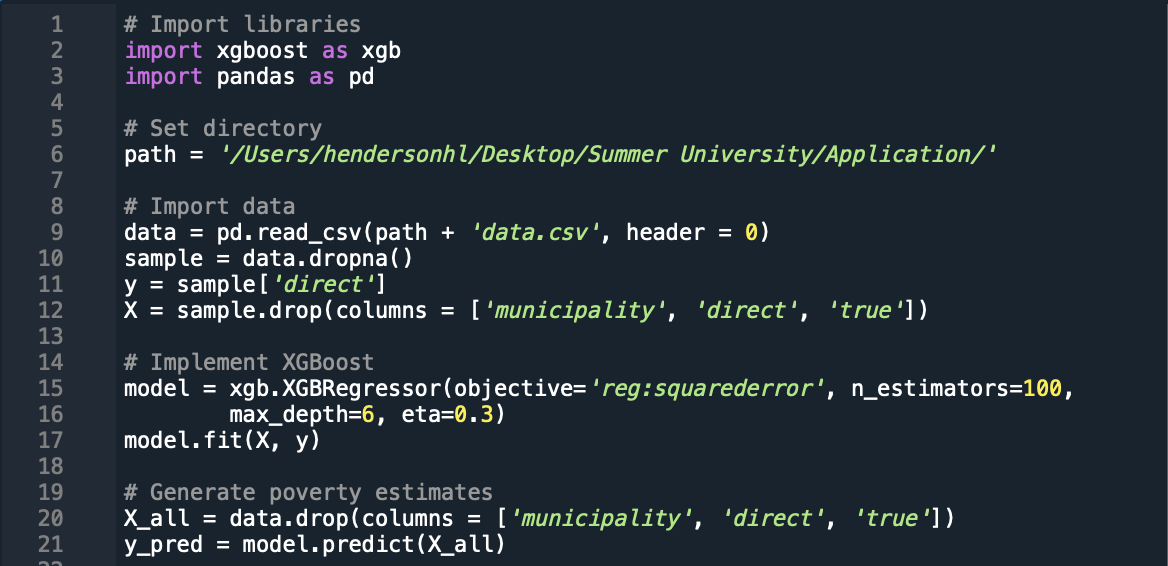
\includegraphics[width=0.8 \textwidth]{Code_1}
\end{figure}
\end{frame}

% An Application
\begin{frame}{An Application}
\begin{figure}[h!]
  \centering
  \includegraphics[width=0.5 \textwidth]{split}
\end{figure}
\end{frame}

% An Application
\begin{frame}{An Application}
\begin{figure}[h!]
  \centering
  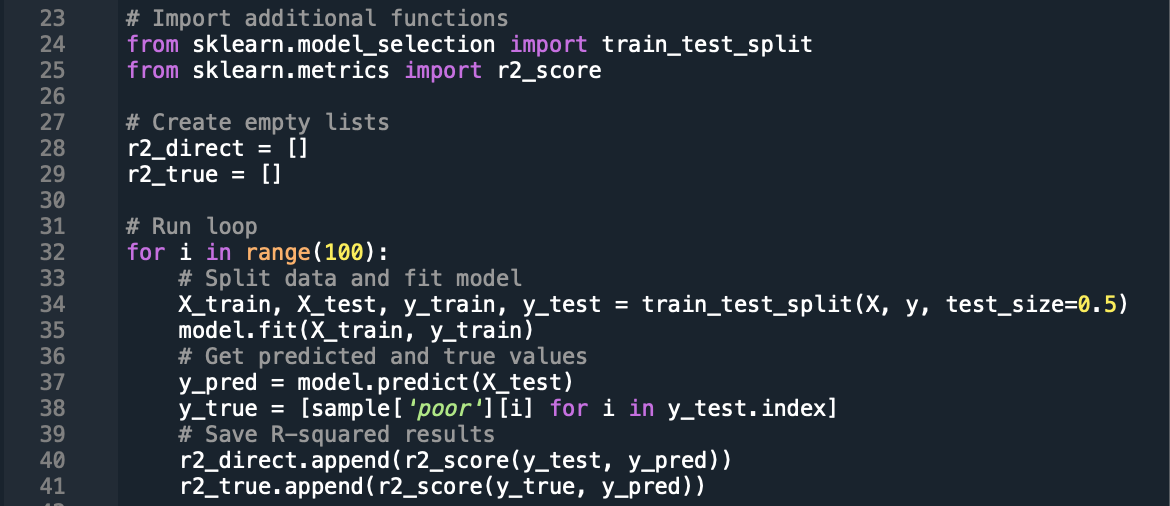
\includegraphics[width=0.8 \textwidth]{Code_2}
\end{figure}
\end{frame}

% An Application
\begin{frame}{An Application}
\begin{figure}[h!]
  \centering
  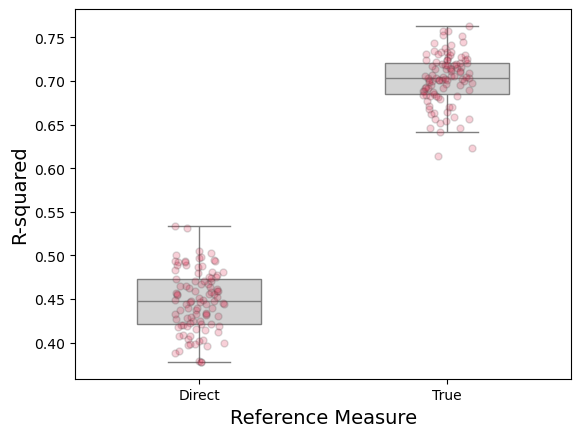
\includegraphics[width=0.6 \textwidth]{Plot}
\end{figure}
\end{frame}

% Resources
\begin{frame}{Resources}
\begin{itemize}
\item Friedman, J.\ (2001). Greedy function approximation: A gradient boosting machine.
\textit{Annals of Statistics}, 29(5): 1189--1232.
\item Chen, T.\ and Guestrin, C.\ (2016). XGBoost: A scalable tree boosting system. In
\textit{Proceedings of the 22nd ACM SIGKDD International Conference on Knowledge 
Discovery and Data Mining}, pages 785--794.
\item Natekin, A.\ and Kroll, A.\ (2013). Gradient boosting machines, a tutorial. 
\textit{Frontiers in Neurorobotics}, 7(21): 1--21.
\item Corral, P., Henderson, H., and Segovia, S. (2023). Poverty mapping in the
age of machine learning. World Bank Policy Research Working Paper No.\ 10429.
\end{itemize}
\end{frame}

\end{document}


















